\section{Results}
\subsection{Initial Analysis}
We discovered that the front-end languages react and angular received a disproportionate number of commits during the initial analysis. These data show a distinct trend in language usage over time, with the number of commits for react decreasing from the year 2015, which was 2656, to the year 2021, which was 778, and the same is valid for angular.
In 2015, there were 3364 commits, and by 2021, that number will have dropped to 2278.

Compared to other front end languages, these two languages received the most significant number of commits because they were both the most ancient languages. During those years, most front-end applications relied solely on these programming languages to achieve their functionality.

The vue language had the lowest number of commits compared to all other languages. This is because it is a new developing language and people are more familiar with the front end languages they use from the beginning.

According to the data in all of the graphs, the number of open issues for Angular was the highest compared to all other languages, and the same was true for the number of closed issues. When it comes to frontend languages, Angular is most commonly used, and a wide range of applications supports it. Despite this, the number of open issues for new languages has increased in the years following 2019. We can assume that people started working on these languages because they offer better scalability, performance, security, and other advantages over react and angular.

\subsection{Answers}
\subsubsection{Is the project alive?}
We are going to use \textbf{time} as the basis to which we are going to attach the metrics, if we see an increase overtime around a project we could say that a project has an active community and the contributions, which could be issues or commits, are increasing over time, otherwise if we see a decline we can see how steep this decline is, and raise that so the contributor take that into consideration.

\paragraph{Trend of commits over the years:} 

We use the following data set \cite{trend-of-commits-over-the-years} that count all the commits that were performed for each project each year and we plot it in the chart below.
\begin{center}
    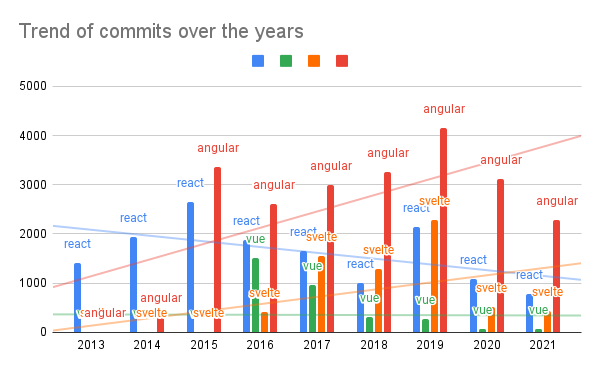
\includegraphics[scale=0.35]{trend-of-commits-over-the-years}    
\end{center}

We can see that for react an increase in the first 3 years but after that there has been a decline in the amount of commits, on the other hand we can see that angular started one year later after react and it surpass it in 2015, and the rate of commits has been increasing ever since.

Vue and Svelte are the newest framework, both conceive in 2016, vue's contribution has been more stable over the last few year while svelte has a trend of increasing, and the amount of commits seems to surpassed vue most years.

Even tough react is the only project that has a declining trendline we don't think that is dying, if we take a look at the table provided in the section \textit{Current state of the world}, react is used by 7.6 million projects.

We can't take react outside of the context on which it was born, inside Facebook, to standarize the way that developers create user interfaces, we attribute this decline to the maturity of the framework, using the Capability maturity model \cite{cmm}, tell us that the project is at level 5, and their focus right now is to improve performance while keeping the stability of the project.

\paragraph{Trend of opened issues over the years: }
The last trend tell us how developers interact with the project, while this trend emphasizes how the community interacts with the project, issues are the social component in open source, at least in github.

In the following chart we did the same approach as before, we take all the date where the issues were open and we group them by year, and we put the projects next to each other to get any insights, below we have a chart that depict a summary of the issues over the years, for this we use the following data set \cite{trend-of-open-issues-over-the-years}.

\begin{center}
    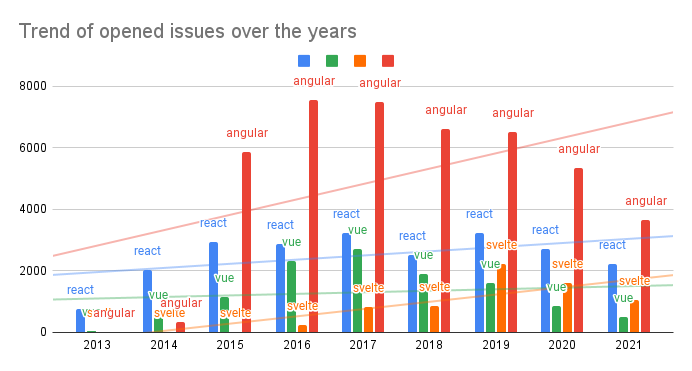
\includegraphics[scale=0.35]{trend-of-open-issues-over-the-years}    
\end{center}

From the following chart we can see that angular has the most active community overall, from react we can see that we have an increasing trendline over the years, which contrast with the decline that it's perceive from the previous trend, which helps with the assumption that we make before that commit's alone are not a single representative metric that provide \textit{liveliness} to a project, vue has a slightly increase over the years and has the same trend behaviour that was displayed in the previous trend, svelte seems to have a increase trendline as well, surpassing vue community in the last 3 years.

This could tell us that overall, all of this communities are fairly active which suggest that the project is alive, from an social aspect.

\paragraph{Trend of unique contributors per year}
We already saw the amount of contributions a code received, in the form of commits, and how the community interact with each other, now are we going to see how big the community is by the amount of unique developers that contribute to the project, we are going to use the following data set\cite{trend-of-unique-contributors-per-year} to create the chart that is shown below.

\begin{center}
    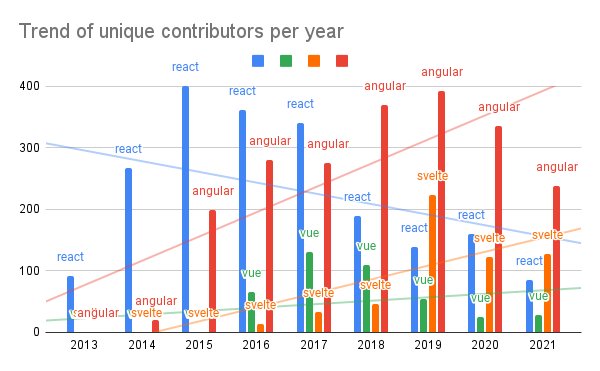
\includegraphics[scale=0.35]{trend-of-unique-contributors-per-year}    
\end{center}

From the chart we can see a decline in react from 2015 to 2021, it could be because at the beggining more developers were joining but with the pass of time the community was getting more mature and the contributions got centralized which coincide with the trend of commits over the years, angular has receive an increase in unique contributors each years which is a sign that the amount of developers is growing, svelte has seen an increase in the last years and vue has receive a fairly increase of contributors since it's inception.

\subsubsection{What is the overall sentiment of the project?}
Now we are going to evaluate what are the positive and negative sentiments for each project, using the following data \cite{overall-sentiment}.

Below we are going to see a chart that depict what is the percentage of positive and negative words used in each projects.

\begin{center}
    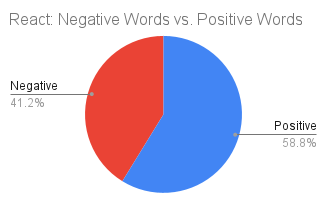
\includegraphics[scale=0.5]{react-words}    
\end{center}

In this chart we can see that react has more positive (162,415) words that represents 58.8\% compare to the negative (113,892) words, which represents 41.2\%.

\begin{center}
    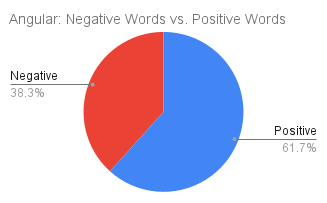
\includegraphics[scale=0.50]{angular-words}    
\end{center}

In the case of angular we have a more positive community than react with 280,779 positive words, which represents a 61.7\%, compare with the 174,500 negative words which represents the 38.3\%.

\begin{center}
    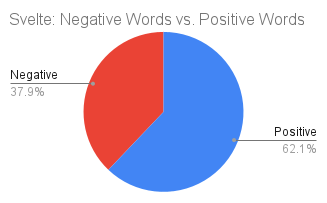
\includegraphics[scale=0.50]{svelte-words}    
\end{center}

Next we have svelte with 35,965 positive words that represents the 62.1\% and 21,948 negative words that represents the 37.9\%.

\begin{center}
    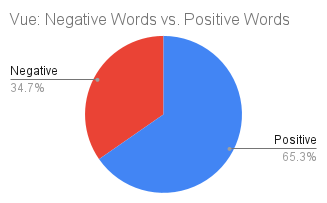
\includegraphics[scale=0.50]{vue-words}    
\end{center}

Vue has a total of 44,901 positive words, 65.3\%, and 23,821 negative words, 34.7\%.

This informations suggest that all the communities are positive in general, and there are big differences between each other, now we are going to display what are the most used words, top 20, using cloud words and for each project we are going to see if it gives us an indication of what the community looks like.

\begin{center}
    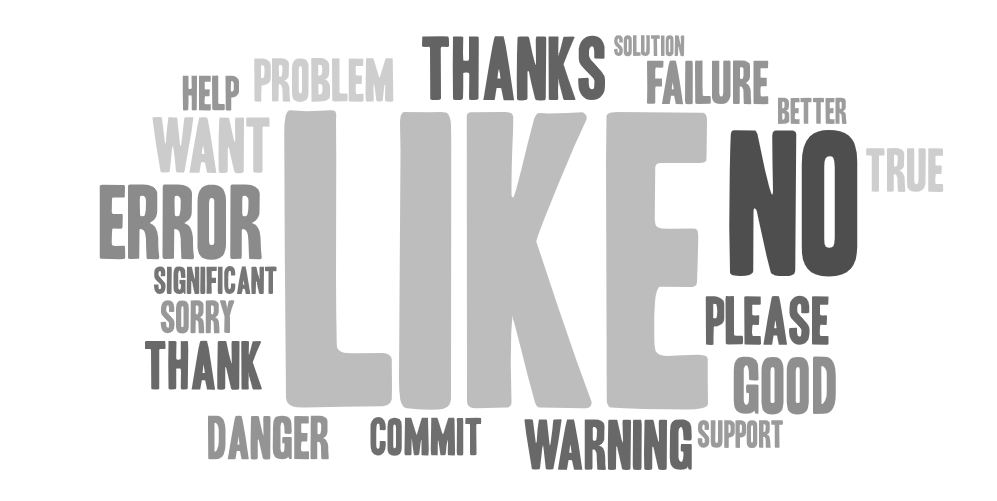
\includegraphics[scale=0.20]{react-word-cloud}    
    \textit{React}
\end{center}


\begin{center}
    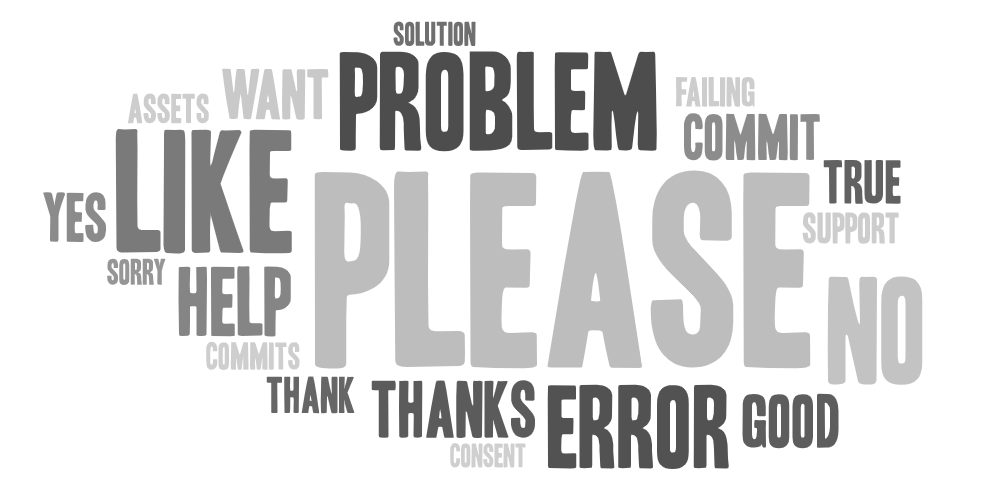
\includegraphics[scale=0.20]{angular-word-cloud}    
    \textit{Angular}
\end{center}


\begin{center}
    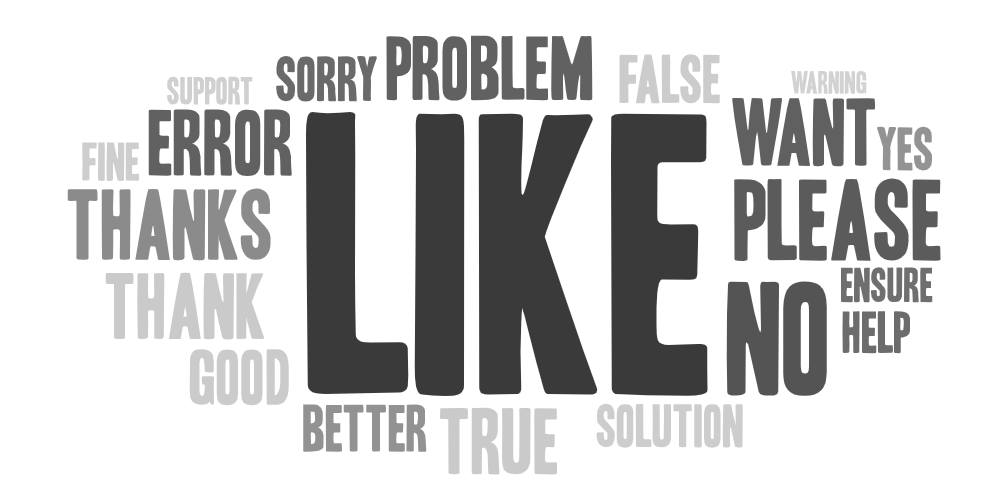
\includegraphics[scale=0.20]{vue-word-cloud}    
    \textit{Vue}
\end{center}

\begin{center}
    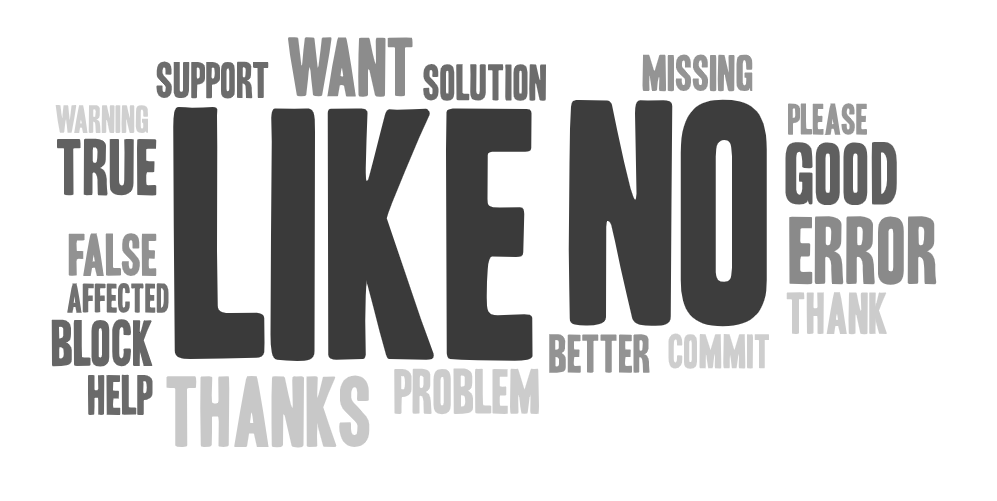
\includegraphics[scale=0.20]{svelte-word-cloud}    
    \textit{Svelte}
\end{center}

From the cloud words we can see that the most use words is \textbf{Like} and \textbf{Please}, and most uses get used accross multiple projects like \textbf{thanks}, \textbf{thank}, \textbf{good}, \textbf{no}, \textbf{problem}, which suggest that there is not a specific words that difference one community from another and overall all the communities are positive, because if we take a look at the negative words are words like \textbf{no}, \textbf{danger} or \textbf{problem} which could for fixing a particular problem.


